% Created 2025-10-16 Thu 21:19
% Intended LaTeX compiler: lualatex
\documentclass[11pt]{article}
\usepackage{amsmath}
\usepackage{fontspec}
\usepackage{graphicx}
\usepackage{longtable}
\usepackage{wrapfig}
\usepackage{rotating}
\usepackage[normalem]{ulem}
\usepackage{capt-of}
\usepackage{hyperref}
\usepackage{booktabs}
\usepackage{upquote}
\usepackage{fvextra}
\usepackage[latte,styleAll]{catppuccinpalette} \setlength{\parindent}{0pt}  \usepackage{hyperref} \usepackage{scrextend} \usepackage{fvextra} \usepackage{upquote} \usepackage{xcolor}  \hypersetup{colorlinks=false, hidelinks=true} \usepackage{circuitikz} \usepackage{rotating}  \usepackage{tabularx, colortbl} \usepackage{geometry}  \newgeometry{vmargin={22mm}, hmargin={22mm,22mm}}
\usepackage{sectsty} \sectionfont{\centering}  %To center heading
\date{\today}
\title{}
\hypersetup{
 pdfauthor={},
 pdftitle={},
 pdfkeywords={},
 pdfsubject={},
 pdfcreator={},
 pdflang={English}}

% Setup for code blocks [1/2]

\usepackage{fvextra}

\fvset{%
  commandchars=\\\{\},
  highlightcolor=white!95!black!80!blue,
  breaklines=true,
  breaksymbol=\color{white!60!black}\tiny\ensuremath{\hookrightarrow}}

% Make line numbers smaller and grey.
\renewcommand\theFancyVerbLine{\footnotesize\color{black!40!white}\arabic{FancyVerbLine}}

\usepackage{xcolor}

% In case engrave-faces-latex-gen-preamble has not been run.
\providecolor{EfD}{HTML}{f7f7f7}
\providecolor{EFD}{HTML}{28292e}

% Define a Code environment to prettily wrap the fontified code.
\usepackage[breakable,xparse]{tcolorbox}
\DeclareTColorBox[]{Code}{o}%
{colback=EfD!98!EFD, colframe=EfD!95!EFD,
  fontupper=\footnotesize\setlength{\fboxsep}{0pt},
  colupper=EFD,
  IfNoValueTF={#1}%
  {boxsep=2pt, arc=2.5pt, outer arc=2.5pt,
    boxrule=0.5pt, left=2pt}%
  {boxsep=2.5pt, arc=0pt, outer arc=0pt,
    boxrule=0pt, leftrule=1.5pt, left=0.5pt},
  right=2pt, top=1pt, bottom=0.5pt,
  breakable}

% Support listings with captions
\usepackage{float}
\floatstyle{plain}
\newfloat{listing}{htbp}{lst}
\newcommand{\listingsname}{Listing}
\floatname{listing}{\listingsname}
\newcommand{\listoflistingsname}{List of Listings}
\providecommand{\listoflistings}{\listof{listing}{\listoflistingsname}}


% Setup for code blocks [2/2]: syntax highlighting colors

\newcommand\efstrut{\vrule height 2.1ex depth 0.8ex width 0pt}
\definecolor{EFD}{HTML}{4c4f69}
\definecolor{EfD}{HTML}{eff1f5}
\newcommand{\EFD}[1]{\textcolor{EFD}{#1}} % default
\newcommand{\EFvp}[1]{#1} % variable-pitch
\definecolor{EFh}{HTML}{bcc0cc}
\newcommand{\EFh}[1]{\textcolor{EFh}{#1}} % shadow
\definecolor{EFsc}{HTML}{40a02b}
\newcommand{\EFsc}[1]{\textcolor{EFsc}{\textbf{#1}}} % success
\definecolor{EFw}{HTML}{fe640b}
\newcommand{\EFw}[1]{\textcolor{EFw}{\textbf{#1}}} % warning
\definecolor{EFe}{HTML}{d20f39}
\newcommand{\EFe}[1]{\textcolor{EFe}{\textbf{#1}}} % error
\definecolor{EFl}{HTML}{1e66f5}
\newcommand{\EFl}[1]{\textcolor{EFl}{\textbf{#1}}} % link
\definecolor{EFlv}{HTML}{8839ef}
\newcommand{\EFlv}[1]{\textcolor{EFlv}{#1}} % link-visited
\definecolor{EFhi}{HTML}{414868}
\definecolor{Efhi}{HTML}{e6e9ef}
\newcommand{\EFhi}[1]{\colorbox{Efhi}{\efstrut{}\textcolor{EFhi}{#1}}} % highlight
\definecolor{EFc}{HTML}{bcc0cc}
\newcommand{\EFc}[1]{\textcolor{EFc}{#1}} % font-lock-comment-face
\definecolor{EFcd}{HTML}{bcc0cc}
\newcommand{\EFcd}[1]{\textcolor{EFcd}{#1}} % font-lock-comment-delimiter-face
\definecolor{EFs}{HTML}{40a02b}
\newcommand{\EFs}[1]{\textcolor{EFs}{#1}} % font-lock-string-face
\definecolor{EFd}{HTML}{acb0be}
\newcommand{\EFd}[1]{\textcolor{EFd}{#1}} % font-lock-doc-face
\definecolor{EFm}{HTML}{fe640b}
\newcommand{\EFm}[1]{\textcolor{EFm}{#1}} % font-lock-doc-markup-face
\definecolor{EFk}{HTML}{8839ef}
\newcommand{\EFk}[1]{\textcolor{EFk}{#1}} % font-lock-keyword-face
\definecolor{EFb}{HTML}{179299}
\newcommand{\EFb}[1]{\textcolor{EFb}{#1}} % font-lock-builtin-face
\definecolor{EFf}{HTML}{1e66f5}
\newcommand{\EFf}[1]{\textcolor{EFf}{#1}} % font-lock-function-name-face
\definecolor{EFv}{HTML}{d20f39}
\newcommand{\EFv}[1]{\textcolor{EFv}{#1}} % font-lock-variable-name-face
\definecolor{EFt}{HTML}{df8e1d}
\newcommand{\EFt}[1]{\textcolor{EFt}{#1}} % font-lock-type-face
\definecolor{EFo}{HTML}{fe640b}
\newcommand{\EFo}[1]{\textcolor{EFo}{#1}} % font-lock-constant-face
\definecolor{EFwr}{HTML}{d20f39}
\newcommand{\EFwr}[1]{\textcolor{EFwr}{\textbf{#1}}} % font-lock-warning-face
\definecolor{EFnc}{HTML}{40a02b}
\newcommand{\EFnc}[1]{\textcolor{EFnc}{\textbf{#1}}} % font-lock-negation-char-face
\definecolor{EFpp}{HTML}{1e66f5}
\newcommand{\EFpp}[1]{\textcolor{EFpp}{\textbf{#1}}} % font-lock-preprocessor-face
\definecolor{EFrc}{HTML}{8839ef}
\newcommand{\EFrc}[1]{\textcolor{EFrc}{\textbf{#1}}} % font-lock-regexp-grouping-construct
\definecolor{EFrb}{HTML}{df8e1d}
\newcommand{\EFrb}[1]{\textcolor{EFrb}{\textbf{#1}}} % font-lock-regexp-grouping-backslash
\definecolor{Efob}{HTML}{e6e9ef}
\newcommand{\EFob}[1]{\colorbox{Efob}{\efstrut{}#1}} % org-block
\definecolor{EFobb}{HTML}{bcc0cc}
\definecolor{Efobb}{HTML}{e6e9ef}
\newcommand{\EFobb}[1]{\colorbox{Efobb}{\efstrut{}\textcolor{EFobb}{#1}}} % org-block-begin-line
\definecolor{EFobe}{HTML}{bcc0cc}
\definecolor{Efobe}{HTML}{e6e9ef}
\newcommand{\EFobe}[1]{\colorbox{Efobe}{\efstrut{}\textcolor{EFobe}{#1}}} % org-block-end-line
\definecolor{EFOa}{HTML}{7aa2f7}
\newcommand{\EFOa}[1]{\textcolor{EFOa}{\textbf{#1}}} % outline-1
\definecolor{EFOb}{HTML}{bb9af7}
\newcommand{\EFOb}[1]{\textcolor{EFOb}{\textbf{#1}}} % outline-2
\definecolor{EFOc}{HTML}{9aa5ce}
\newcommand{\EFOc}[1]{\textcolor{EFOc}{\textbf{#1}}} % outline-3
\definecolor{EFOd}{HTML}{9bb9f9}
\newcommand{\EFOd}[1]{\textcolor{EFOd}{\textbf{#1}}} % outline-4
\definecolor{EFOe}{HTML}{cbb3f9}
\newcommand{\EFOe}[1]{\textcolor{EFOe}{\textbf{#1}}} % outline-5
\definecolor{EFOf}{HTML}{bcd0fb}
\newcommand{\EFOf}[1]{\textcolor{EFOf}{\textbf{#1}}} % outline-6
\definecolor{EFOg}{HTML}{ddccfb}
\newcommand{\EFOg}[1]{\textcolor{EFOg}{\textbf{#1}}} % outline-7
\definecolor{EFOh}{HTML}{e4ecfd}
\newcommand{\EFOh}[1]{\textcolor{EFOh}{\textbf{#1}}} % outline-8
\newcommand{\EFhn}[1]{#1} % highlight-numbers-number
\newcommand{\EFhq}[1]{#1} % highlight-quoted-quote
\newcommand{\EFhs}[1]{#1} % highlight-quoted-symbol
\definecolor{EFrda}{HTML}{8839ef}
\newcommand{\EFrda}[1]{\textcolor{EFrda}{#1}} % rainbow-delimiters-depth-1-face
\definecolor{EFrdb}{HTML}{1e66f5}
\newcommand{\EFrdb}[1]{\textcolor{EFrdb}{#1}} % rainbow-delimiters-depth-2-face
\definecolor{EFrdc}{HTML}{179299}
\newcommand{\EFrdc}[1]{\textcolor{EFrdc}{#1}} % rainbow-delimiters-depth-3-face
\definecolor{EFrdd}{HTML}{40a02b}
\newcommand{\EFrdd}[1]{\textcolor{EFrdd}{#1}} % rainbow-delimiters-depth-4-face
\definecolor{EFrde}{HTML}{df8e1d}
\newcommand{\EFrde}[1]{\textcolor{EFrde}{#1}} % rainbow-delimiters-depth-5-face
\definecolor{EFrdf}{HTML}{fe640b}
\newcommand{\EFrdf}[1]{\textcolor{EFrdf}{#1}} % rainbow-delimiters-depth-6-face
\definecolor{EFrdg}{HTML}{d20f39}
\newcommand{\EFrdg}[1]{\textcolor{EFrdg}{#1}} % rainbow-delimiters-depth-7-face
\definecolor{EFrdh}{HTML}{bcc0cc}
\newcommand{\EFrdh}[1]{\textcolor{EFrdh}{#1}} % rainbow-delimiters-depth-8-face
\newcommand{\EFrdi}[1]{#1} % rainbow-delimiters-depth-9-face
\definecolor{EFany}{HTML}{df8e1d}
\definecolor{Efany}{HTML}{df8e1d}
\newcommand{\EFany}[1]{\colorbox{Efany}{\efstrut{}\textcolor{EFany}{#1}}} % ansi-color-yellow
\definecolor{EFanr}{HTML}{d20f39}
\definecolor{Efanr}{HTML}{d20f39}
\newcommand{\EFanr}[1]{\colorbox{Efanr}{\efstrut{}\textcolor{EFanr}{#1}}} % ansi-color-red
\definecolor{EFanb}{HTML}{ccd0da}
\newcommand{\EFanb}[1]{\textcolor{EFanb}{#1}} % ansi-color-black
\definecolor{EFang}{HTML}{40a02b}
\definecolor{Efang}{HTML}{40a02b}
\newcommand{\EFang}[1]{\colorbox{Efang}{\efstrut{}\textcolor{EFang}{#1}}} % ansi-color-green
\definecolor{EFanB}{HTML}{1e66f5}
\definecolor{EfanB}{HTML}{1e66f5}
\newcommand{\EFanB}[1]{\colorbox{EfanB}{\efstrut{}\textcolor{EFanB}{#1}}} % ansi-color-blue
\definecolor{EFanc}{HTML}{179299}
\definecolor{Efanc}{HTML}{179299}
\newcommand{\EFanc}[1]{\colorbox{Efanc}{\efstrut{}\textcolor{EFanc}{#1}}} % ansi-color-cyan
\definecolor{Efanw}{HTML}{7287fd}
\newcommand{\EFanw}[1]{\colorbox{Efanw}{\efstrut{}#1}} % ansi-color-white
\definecolor{EFanm}{HTML}{8839ef}
\definecolor{Efanm}{HTML}{8839ef}
\newcommand{\EFanm}[1]{\colorbox{Efanm}{\efstrut{}\textcolor{EFanm}{#1}}} % ansi-color-magenta
\definecolor{EFANy}{HTML}{e4bb7e}
\definecolor{EfANy}{HTML}{e4bb7e}
\newcommand{\EFANy}[1]{\colorbox{EfANy}{\efstrut{}\textcolor{EFANy}{#1}}} % ansi-color-bright-yellow
\definecolor{EFANr}{HTML}{f88a9e}
\definecolor{EfANr}{HTML}{f88a9e}
\newcommand{\EFANr}[1]{\colorbox{EfANr}{\efstrut{}\textcolor{EFANr}{#1}}} % ansi-color-bright-red
\definecolor{EFANb}{HTML}{a0aad2}
\definecolor{EfANb}{HTML}{a0aad2}
\newcommand{\EFANb}[1]{\colorbox{EfANb}{\efstrut{}\textcolor{EFANb}{#1}}} % ansi-color-bright-black
\definecolor{EFANg}{HTML}{88dfd1}
\definecolor{EfANg}{HTML}{88dfd1}
\newcommand{\EFANg}[1]{\colorbox{EfANg}{\efstrut{}\textcolor{EFANg}{#1}}} % ansi-color-bright-green
\definecolor{EFANB}{HTML}{8daff8}
\definecolor{EfANB}{HTML}{8daff8}
\newcommand{\EFANB}[1]{\colorbox{EfANB}{\efstrut{}\textcolor{EFANB}{#1}}} % ansi-color-bright-blue
\definecolor{EFANc}{HTML}{bff9f9}
\definecolor{EfANc}{HTML}{bff9f9}
\newcommand{\EFANc}[1]{\colorbox{EfANc}{\efstrut{}\textcolor{EFANc}{#1}}} % ansi-color-bright-cyan
\definecolor{EFANw}{HTML}{c0caf5}
\definecolor{EfANw}{HTML}{c0caf5}
\newcommand{\EFANw}[1]{\colorbox{EfANw}{\efstrut{}\textcolor{EFANw}{#1}}} % ansi-color-bright-white
\definecolor{EFANm}{HTML}{c5a9f8}
\definecolor{EfANm}{HTML}{c5a9f8}
\newcommand{\EFANm}[1]{\colorbox{EfANm}{\efstrut{}\textcolor{EFANm}{#1}}} % ansi-color-bright-magenta
\begin{document}

\begin{center}

\includegraphics[width=.9\linewidth]{../killdozer.png}
\end{center}
\section*{{\color{CtpPink} ELEC3020 Project Design Report}}
\label{sec:org3be1770}
\section*{{\color{CtpPink} Team-27 }}
\label{sec:org9984cba}

\vspace{25mm}
\textbf{Signed by:}\\
\vspace{5mm}

Mia O'Dea \\
Sebastian Gazey\\
Sophie Mattingly\\
Carla Schultz\\

\clearpage
\subsection*{\textbf{Introduction}}
\label{sec:orgdced49a}
The objective of the project is to create a SumoBot using the ESP32 TTGO microcontroller.
The robot is designed to detect, engage, and push other robot opponents outside a circular ring, while remaining within the white boundary line.
The project enforces practical implementation of the concepts learnt in the Embedded Systems (ELEC3020) unit.\\

This report documents the complete design, development, and implementation of the custom built SumoBot “KillDozer”.
\subsection*{Team Contributions}
\label{sec:org9810dfb}
The parts that each team member worked on is below:
\begin{table}[htbp]
\caption{Team Member Contributions}
\centering
\begin{tabularx}{\textwidth}{|X|X|}
\toprule
\textbf{Team Member (Student Number)} & \textbf{Contributions}\\
\midrule
Sebastian Gazey (23417131) & Design Decisions\\
 & Project Design Report\\
 & Software (both strategy and writing the code)\\
 & Chassis/Parts Design\\
 & Electronics (purchasing, research, design, assembly/soldering)\\
 & Assembly\\
 & 3D printing\\
 & Testing\\
 & Bill of Materials\\
\midrule
Mia O'Dea (23729581) & Design Decisions\\
 & Chassis/Parts Design\\
 & Project Design Report\\
 & Electronics (soldering, design)\\
 & Assembly\\
 & 3D printing\\
 & Testing\\
 & Bill of Materials\\
\midrule
Carla Schultz (23854485) & Bill of Materials\\
 & User Manual\\
 & Marketing Document\\
 & Project Design Report\\
\midrule
Sophie Mattingly (23771898) & Bill of Materials\\
 & User Manual\\
 & Marketing Document\\
 & Project Design Report\\
\bottomrule
\end{tabularx}
\end{table}
\subsection*{Design Choices}
\label{sec:orge2fd762}
There were a few key principles that KillDozer was built around, these being maintaining traction, detection (of opponents and the competition area), and flipping/pushing the opponent.
\subsubsection*{Traction}
\label{sec:orga294891}
A large surface area was crucial to maintaining traction, and as such, KillDozer uses two tracks as the driving system. These had the added benefit of increasing the agility of KillDozer, as differential steering could be used, allowing it to turn on the spot - this system also had the added benefit of reducing the complexity of the steering system (as a separate servo to control a steering axle was not needed).\\

To increase traction even more, KillDozer was going to have Dycem\textsuperscript{tm} attached to the tracks (however, the team ran out of time to implement this).
\subsubsection*{Detection}
\label{sec:org8c9292a}
KillDozer uses two URM09 ultrasonic sensors as the main way to detect opponents. These were chosen due to having a wider field of view than HC-SR04's.\\

There are also RGB colour sensors at the front two corners, to detect if the robot is about to drive out of the circle.
\begin{figure}[htbp]
\centering

\includegraphics[width=4in]{/home/bones/Storage/Uniwork/.gitJankness/ELEC3020_Project/RGBSensors.JPG}
\caption{RGB sensors underneath the blade}
\end{figure}
\subsubsection*{Pushing/Flipping}
\label{sec:org8201b35}
For this KillDozer has a bulldozer like blade - this has gone through numerous iterations to save weight, the final version:
\begin{figure}[htbp]
\centering

\includegraphics[width=4in]{/home/bones/Storage/Uniwork/.gitJankness/ELEC3020_Project/bladenew.jpg}
\caption{Bulldozer blade, with URM09 sensors}
\end{figure}
\subsection*{Hardware:}
\label{sec:org0d57bb2}
\subsubsection*{Circuit Diagram:}
\label{sec:orgde6fa4e}
\begin{turn}{90}
\usetikzlibrary{shapes.geometric}
\begin{tikzpicture}
	% Paths, nodes and wires:
	\node[shape=rectangle, rotate=-90, draw, line width=1pt, dash pattern={on 4pt off 2pt}, minimum width=2.465cm, minimum height=6.965cm] at (25.386, -0.25){};
	\node[shape=ellipse, rotate=-90, draw, line width=1pt, minimum width=1.236cm, minimum height=1.215cm] at (27.558, -0.864){};
	\node[shape=rectangle, draw, line width=1pt, dash pattern={on 4pt off 2pt}, minimum width=3.715cm, minimum height=6.715cm] at (18.125, 9.5){};
	\node[shape=rectangle, draw, line width=1pt, dash pattern={on 4pt off 2pt}, minimum width=3.715cm, minimum height=7.715cm] at (8.125, 4.625){};
	\node[shape=rectangle, draw, line width=1pt, minimum width=3.465cm, minimum height=7.215cm] at (12.813, 5.25){};
	\node[shape=rectangle, minimum width=1.465cm, minimum height=0.715cm] at (12.813, 8.375){} node[anchor=north, align=center, text width=1.077cm, inner sep=6pt] at (12.813, 8.75){LILYGO};
	\node[shape=ellipse, draw, line width=1pt, minimum width=0.715cm, minimum height=0.465cm] at (11.813, 2){};
	\node[shape=ellipse, draw, line width=1pt, minimum width=0.715cm, minimum height=0.465cm] at (13.812, 2){};
	\draw (10.563, 8) -- (11.312, 8);
	\draw (10.563, 7.5) -- (11.312, 7.5);
	\path[draw={CtpMauve}] (10.563, 7) -- (11.312, 7);
	\path[draw={CtpPeach}] (10.563, 6.5) -- (11.312, 6.5);
	\path[draw={CtpPink}] (10.563, 5) -- (11.312, 5);
	\path[draw={CtpBlue}] (10.563, 4.5) -- (11.312, 4.5);
	\draw (10.563, 4) -- (11.312, 4);
	\draw (10.563, 3.5) -- (11.312, 3.5);
	\draw (10.563, 3) -- (11.312, 3);
	\draw (10.563, 2.5) -- (11.312, 2.5);
	\draw (14.313, 8) -- (15.062, 8);
	\draw (14.313, 7.5) -- (15.062, 7.5);
	\draw (14.313, 7) -- (15.062, 7);
	\draw (14.313, 6.5) -- (15.062, 6.5);
	\path[draw={CtpSky}] (14.313, 6) -- (15.062, 6);
	\path[draw={CtpGreen}] (14.313, 5.5) -- (15.062, 5.5);
	\path[draw={CtpLavender}] (14.313, 5) -- (15.062, 5);
	\path[draw={CtpTeal}] (14.313, 4.5) -- (15.062, 4.5);
	\draw (14.313, 4) -- (15.062, 4);
	\draw (14.313, 3.5) -- (15.062, 3.5);
	\path[draw={rgb,255:red,17;green,17;blue,27}] (14.313, 3) -- (15.75, 3);
	\path[draw={CtpRed}] (14.313, 2.5) -| (16, 2.5);
	\node[waves, xscale=-1.04, yscale=-1.04] at (7.298, 5.5){};
	\path[draw={rgb,255:red,17;green,17;blue,27}] (10.75, 0.5) |- (10.25, 1.75) |- (8, 6.25);
	\path[draw={CtpFlamingo}] (11.062, 5.5) -| (8.25, 5.5) |- (8, 5.25);
	\path[draw={CtpYellow}] (10.875, 6) -| (8.25, 6) -- (8.25, 5.75) -- (8, 5.75);
	\path[draw={CtpRed}] (8, 4.75) |- (9.75, 4.688);
	\path[draw={CtpRed}] (10.25, 1.25) -- (10.25, 0.25) -| (16, 2.5);
	\node[shape=rectangle, minimum width=2.715cm, minimum height=1.715cm] at (7.625, 7.625){} node[anchor=north west, align=left, text width=2.327cm, inner sep=6pt] at (6.25, 8.5){\Large Ultrasonic Sensors};
	\node[shape=rectangle, minimum width=1.871cm, minimum height=0.465cm] at (13.703, 2.5){} node[anchor=center, align=center, text width=1.483cm, inner sep=6pt] at (13.703, 2.5){\small 5V};
	\node[shape=rectangle, minimum width=1.715cm, minimum height=0.465cm] at (11.875, 5){} node[anchor=center, align=center, text width=1.327cm, inner sep=6pt] at (11.875, 5){\small PIN 21};
	\node[shape=rectangle, minimum width=1.715cm, minimum height=0.465cm] at (11.875, 4.5){} node[anchor=center, align=center, text width=1.327cm, inner sep=6pt] at (11.875, 4.5){\small PIN 16};
	\node[shape=rectangle, minimum width=1.715cm, minimum height=0.465cm] at (11.875, 4){} node[anchor=center, align=center, text width=1.327cm, inner sep=6pt] at (11.875, 4){\small NC};
	\node[shape=rectangle, minimum width=1.715cm, minimum height=0.465cm] at (11.875, 3.5){} node[anchor=center, align=center, text width=1.327cm, inner sep=6pt] at (11.875, 3.5){\small GND};
	\node[shape=rectangle, minimum width=1.715cm, minimum height=0.465cm] at (11.875, 3){} node[anchor=center, align=center, text width=1.327cm, inner sep=6pt] at (11.875, 3){\small GND};
	\node[shape=rectangle, minimum width=1.715cm, minimum height=0.465cm] at (11.875, 2.5){} node[anchor=center, align=center, text width=1.327cm, inner sep=6pt] at (11.875, 2.5){\small 3V};
	\node[shape=rectangle, minimum width=1.871cm, minimum height=0.465cm] at (13.703, 3){} node[anchor=center, align=center, text width=1.483cm, inner sep=6pt] at (13.703, 3){\small GND};
	\node[shape=rectangle, minimum width=1.808cm, minimum height=0.465cm] at (11.922, 8){} node[anchor=center, align=center, text width=1.42cm, inner sep=6pt] at (11.922, 8){\small GND};
	\node[shape=rectangle, minimum width=1.808cm, minimum height=0.465cm] at (11.922, 7.5){} node[anchor=center, align=center, text width=1.42cm, inner sep=6pt] at (11.922, 7.5){\small GND};
	\node[shape=rectangle, minimum width=1.715cm, minimum height=0.465cm] at (11.875, 7){} node[anchor=center, align=center, text width=1.327cm, inner sep=6pt] at (11.875, 7){\small PIN 43};
	\node[shape=rectangle, minimum width=1.715cm, minimum height=0.465cm] at (11.875, 6.5){} node[anchor=center, align=center, text width=1.327cm, inner sep=6pt] at (11.875, 6.5){\small PIN 44};
	\node[shape=rectangle, minimum width=1.715cm, minimum height=0.465cm] at (11.875, 6){} node[anchor=center, align=center, text width=1.327cm, inner sep=6pt] at (11.875, 6){\small PIN 18};
	\node[shape=rectangle, minimum width=1.715cm, minimum height=0.465cm] at (11.875, 5.5){} node[anchor=center, align=center, text width=1.327cm, inner sep=6pt] at (11.875, 5.5){\small PIN 17};
	\node[shape=rectangle, minimum width=1.777cm, minimum height=0.465cm] at (13.75, 8){} node[anchor=center, align=center, text width=1.389cm, inner sep=6pt] at (13.75, 8){\small 3V};
	\node[shape=rectangle, minimum width=1.777cm, minimum height=0.465cm] at (13.75, 7.5){} node[anchor=center, align=center, text width=1.389cm, inner sep=6pt] at (13.75, 7.5){\small PIN 1};
	\node[shape=rectangle, minimum width=1.777cm, minimum height=0.465cm] at (13.75, 7){} node[anchor=center, align=center, text width=1.389cm, inner sep=6pt] at (13.75, 7){\small PIN 2};
	\node[shape=rectangle, minimum width=1.777cm, minimum height=0.465cm] at (13.75, 6.5){} node[anchor=center, align=center, text width=1.389cm, inner sep=6pt] at (13.75, 6.5){\small PIN 3};
	\node[shape=rectangle, minimum width=1.777cm, minimum height=0.465cm] at (13.75, 6){} node[anchor=center, align=center, text width=1.389cm, inner sep=6pt] at (13.75, 6){\small PIN 10};
	\node[shape=rectangle, minimum width=1.777cm, minimum height=0.465cm] at (13.75, 5.5){} node[anchor=center, align=center, text width=1.389cm, inner sep=6pt] at (13.75, 5.5){\small PIN 11};
	\node[shape=rectangle, minimum width=1.777cm, minimum height=0.465cm] at (13.75, 5){} node[anchor=center, align=center, text width=1.389cm, inner sep=6pt] at (13.75, 5){\small PIN 12};
	\node[shape=rectangle, minimum width=1.777cm, minimum height=0.465cm] at (13.75, 4.5){} node[anchor=center, align=center, text width=1.389cm, inner sep=6pt] at (13.75, 4.5){\small PIN 13};
	\node[shape=rectangle, minimum width=1.871cm, minimum height=0.465cm] at (13.703, 4){} node[anchor=center, align=center, text width=1.483cm, inner sep=6pt] at (13.703, 4){\small NC};
	\node[shape=rectangle, minimum width=1.871cm, minimum height=0.465cm] at (13.703, 3.5){} node[anchor=center, align=center, text width=1.483cm, inner sep=6pt] at (13.703, 3.5){\small NC};
	\node[shape=rectangle, draw, line width=1pt, minimum width=5.965cm, minimum height=5.215cm] at (25.875, 8.375){};
	\node[shape=rectangle, minimum width=4.715cm, minimum height=0.965cm] at (26, 9.25){} node[anchor=center, align=center, text width=4.327cm, inner sep=6pt] at (26, 9.25){\large Motor Driver Board};
	\node[shape=rectangle, minimum width=3.465cm, minimum height=0.965cm] at (12.813, 9.375){} node[anchor=center, align=center, text width=3.077cm, inner sep=6pt] at (12.813, 9.375){TTGO};
	\node[shape=rectangle, draw, line width=1pt, minimum width=0.715cm, minimum height=0.715cm] at (23.75, 6.375){};
	\node[shape=rectangle, draw, line width=1pt, minimum width=0.715cm, minimum height=0.715cm] at (24.5, 6.375){};
	\node[shape=rectangle, draw, line width=1pt, minimum width=0.715cm, minimum height=0.715cm] at (25.5, 6.375){};
	\node[shape=rectangle, draw, line width=1pt, minimum width=0.715cm, minimum height=0.715cm] at (26.25, 6.375){};
	\node[shape=rectangle, draw, line width=1pt, minimum width=0.715cm, minimum height=0.715cm] at (27.25, 6.375){};
	\node[shape=rectangle, draw, line width=1pt, minimum width=0.715cm, minimum height=0.715cm] at (28, 6.375){};
	\path[draw={CtpSky}] (23.5, 11.25) -| (23.5, 10.5);
	\path[draw={CtpGreen}] (24.5, 11.25) -| (24.5, 10.5);
	\path[draw={CtpRed}] (25.5, 11.25) -| (25.5, 10.5);
	\path[draw={rgb,255:red,17;green,17;blue,27}] (26.5, 11.25) -| (26.5, 10.5);
	\path[draw={CtpLavender}] (27.5, 11.25) -| (27.5, 10.5);
	\path[draw={CtpTeal}] (28.25, 11.25) -| (28.25, 10.5);
	\node[shape=rectangle, minimum width=0.965cm, minimum height=0.465cm] at (23.5, 10.25){} node[anchor=center, align=center, text width=0.577cm, inner sep=6pt] at (23.5, 10.25){\small M1A};
	\node[shape=rectangle, minimum width=0.84cm, minimum height=0.465cm] at (27.5, 10.25){} node[anchor=center, align=center, text width=0.452cm, inner sep=6pt] at (27.5, 10.25){\small M1A};
	\node[shape=rectangle, minimum width=0.84cm, minimum height=0.465cm] at (24.5, 10.25){} node[anchor=center, align=center, text width=0.452cm, inner sep=6pt] at (24.5, 10.25){\small M1B};
	\node[shape=rectangle, minimum width=0.84cm, minimum height=0.465cm] at (28.25, 10.25){} node[anchor=center, align=center, text width=0.452cm, inner sep=6pt] at (28.25, 10.25){\small M2B};
	\node[shape=rectangle, minimum width=0.84cm, minimum height=0.465cm] at (25.5, 10.25){} node[anchor=center, align=center, text width=0.452cm, inner sep=6pt] at (25.5, 10.25){\small 5VO};
	\node[shape=rectangle, minimum width=0.84cm, minimum height=0.465cm] at (26.5, 10.25){} node[anchor=center, align=center, text width=0.452cm, inner sep=6pt] at (26.5, 10.25){\small GND};
	\node[shape=rectangle, minimum width=1.215cm, minimum height=0.715cm] at (24.125, 7.125){} node[anchor=center, align=center, text width=0.827cm, inner sep=6pt] at (24.125, 7.125){M1};
	\node[shape=rectangle, minimum width=1.215cm, minimum height=0.715cm] at (27.625, 7.125){} node[anchor=center, align=center, text width=0.827cm, inner sep=6pt] at (27.625, 7.125){M2};
	\node[shape=rectangle, minimum width=0.715cm, minimum height=0.715cm] at (25.5, 7.125){} node[anchor=center, align=center, text width=0.327cm, inner sep=6pt] at (25.5, 7.125){\small VB+};
	\node[shape=rectangle, minimum width=0.59cm, minimum height=0.715cm] at (26.312, 7.125){} node[anchor=center, align=center, text width=0.202cm, inner sep=6pt] at (26.312, 7.125){\small VB-};
	\node[shape=circle, draw, line width=1pt, minimum width=0.715cm] at (23.75, 6.375){};
	\node[shape=circle, draw, line width=1pt, minimum width=0.715cm] at (24.5, 6.375){};
	\node[shape=circle, draw, line width=1pt, minimum width=0.715cm] at (25.5, 6.375){};
	\node[shape=circle, draw, line width=1pt, minimum width=0.715cm] at (26.25, 6.375){};
	\node[shape=circle, draw, line width=1pt, minimum width=0.715cm] at (27.25, 6.375){};
	\node[shape=circle, draw, line width=1pt, minimum width=0.715cm] at (28, 6.375){};
	\draw[line width=2.2pt] (23.75, 6.75) -- (23.75, 6) -- (23.75, 6.375) -- (23.375, 6.375) -- (24.125, 6.375);
	\draw[line width=2.2pt] (24.5, 6.75) -- (24.5, 6) -- (24.5, 6.375) -- (24.125, 6.375) -- (24.875, 6.375);
	\draw[line width=2.2pt] (25.5, 6.75) -- (25.5, 6) -- (25.5, 6.375) -- (25.125, 6.375) -- (25.875, 6.375);
	\draw[line width=2.2pt] (26.25, 6.75) -- (26.25, 6) -- (26.25, 6.375) -- (25.875, 6.375) -- (26.625, 6.375);
	\draw[line width=2.2pt] (27.25, 6.75) -- (27.25, 6) -- (27.25, 6.375) -- (26.875, 6.375) -- (27.625, 6.375);
	\draw[line width=2.2pt] (28, 6.75) -- (28, 6) -- (28, 6.375) -- (27.625, 6.375) -- (28.375, 6.375);
	\path[draw={CtpSky}] (15.062, 6) -| (20.25, 11.5) -| (23.5, 11.25);
	\path[draw={CtpGreen}] (15.062, 5.5) -| (20.75, 5.75) -- (20.75, 12) -| (24.5, 11.25);
	\path[draw={CtpRed}] (16, 3.5) -| (21.75, 12.5) -| (25.5, 11.25);
	\path[draw={rgb,255:red,17;green,17;blue,27}] (15.75, 4) -| (21.25, 13) -| (26.5, 11.25);
	\path[draw={CtpLavender}] (15.062, 5) -| (22.25, 13.5) -| (27.5, 11.25);
	\path[draw={CtpTeal}] (15.062, 4.5) -| (22.75, 14) -| (28.25, 11.25);
	\path[draw={CtpSky}, line width=2pt] (23.75, 6.375) -- (23.75, -0);
	\path[draw={CtpGreen}, line width=2pt] (24.5, 6.375) -| (24.5, -0);
	\path[draw={CtpLavender}, line width=2pt] (27.25, 6.375) -- (27.25, -0);
	\path[draw={CtpTeal}, line width=2pt] (28, 6.375) -| (28, -0);
	\draw (20.25, 1.75) to[battery, l={$11.1V$}, label distance=-0.02cm] (25.75, 1.75);
	\path[draw={CtpRed}, line width=2pt] (25.5, 3) -| (20.25, 1.75);
	\path[draw={rgb,255:red,17;green,17;blue,27}, line width=2pt] (25.75, 1.75) -- (25.75, 1.75) -| (26.25, 6.375);
	\draw (16.5, 1.75) to[sdcdc] (19.25, 1.75);
	\path[draw={CtpRed}] (19.25, 1.75) -- (20.25, 1.75);
	\path[draw={CtpRed}] (16.5, 0.75) -| (13.115, 1.946);
	\path[draw={rgb,255:red,17;green,17;blue,27}] (12.562, 2) |- (18.5, 0.5);
	\node[shape=rectangle, draw, line width=1pt, dash pattern={on 4pt off 1pt on 1pt off 1pt}, minimum width=0.965cm, minimum height=0.465cm] at (12.813, 2){};
	\node[shape=rectangle, minimum width=2.715cm, minimum height=0.465cm] at (17.875, 2.75){} node[anchor=center, align=center, text width=2.327cm, inner sep=6pt] at (17.875, 2.75){\small 5V Buck Convertor};
	\node[shape=ellipse, rotate=-90, draw, line width=1pt, minimum width=1.184cm, minimum height=1.184cm] at (24.14, -0.89){};
	\node[shape=rectangle, minimum width=0.818cm, minimum height=0.818cm] at (24.145, -0.895){} node[anchor=center, align=center, text width=0.43cm, inner sep=6pt] at (24.145, -0.895){\Large M1};
	\path[draw={CtpGreen}, line width=2pt] (25, -1.03) |- (24.75, -1);
	\path[draw={CtpGreen}, line width=2pt] (25, -1) |- (24.5, -0);
	\path[draw={CtpSky}, line width=2pt] (23.28, -0.89) -| (23.53, -0.89);
	\path[draw={CtpSky}, line width=2pt] (23.75, -0) -| (23.28, -0.89);
	\node[shape=rectangle, minimum width=0.849cm, minimum height=0.864cm] at (27.558, -0.864){} node[anchor=center, align=center, text width=0.461cm, inner sep=6pt] at (27.558, -0.864){\Large M2};
	\path[draw={CtpTeal}, line width=2pt] (28.183, -0.864) -- (28.47, -0.864);
	\path[draw={CtpTeal}, line width=2pt] (28.47, -0.864) |- (28, -0);
	\path[draw={CtpLavender}, line width=2pt] (26.933, -0.864) -- (26.75, -0.864);
	\path[draw={CtpLavender}, line width=2pt] (27.25, -0) -| (26.75, -0.864);
	\node[shape=rectangle, minimum width=1.965cm, minimum height=0.715cm] at (22.886, 0.625){} node[anchor=center, align=center, text width=1.577cm, inner sep=6pt] at (22.886, 0.625){\Large Motors};
	\node[shape=rectangle, draw, line width=1pt, minimum width=0.715cm, minimum height=1.965cm] at (7.625, 5.5){};
	\node[shape=rectangle, draw, line width=1pt, minimum width=3.965cm, minimum height=1.965cm] at (13, 11.5){};
	\node[shape=rectangle, minimum width=3.465cm, minimum height=0.465cm] at (13, 11.5){} node[anchor=center, align=center, text width=3.077cm, inner sep=6pt] at (13, 11.5){I2C Multiplexer};
	\draw (11.25, 12.75) -| (11.25, 12.25);
	\draw (11.75, 12.75) -- (11.75, 12.25) -| (11.75, 12.5);
	\draw (12.25, 12.75) -| (12.25, 12.25);
	\draw (12.75, 12.75) -- (12.75, 12.25) -| (12.75, 12.5);
	\path[draw={rgb,255:red,145;green,65;blue,172}] (14.25, 12.75) -| (14.25, 12.25);
	\path[draw={rgb,255:red,226;green,42;blue,195}] (14.75, 12.75) -- (14.75, 12.25) -| (14.75, 12.5);
	\draw (11.25, 10.75) -| (11.25, 10.25);
	\draw (11.75, 10.75) -- (11.75, 10.25) -| (11.75, 10.5);
	\draw (12.25, 10.75) -| (12.25, 10.25);
	\draw (12.75, 10.75) -- (12.75, 10.25) -| (12.75, 10.5);
	\draw (13.25, 10.75) -| (13.25, 10.25);
	\draw (13.75, 10.75) -- (13.75, 10.25) -| (13.75, 10.5);
	\path[draw={rgb,255:red,145;green,65;blue,172}] (14.25, 10.75) -| (14.25, 10.25);
	\path[draw={rgb,255:red,226;green,42;blue,195}] (14.75, 10.75) -- (14.75, 10.125) -| (14.75, 10.5);
	\path[draw={rgb,255:red,17;green,17;blue,27}] (11.25, 12) |- (10.75, 12);
	\path[draw={CtpRed}] (11.25, 11.75) -- (10.75, 11.75) -- (11, 11.75);
	\path[draw={CtpPeach}] (11.25, 11.5) |- (10.75, 11.5);
	\path[draw={CtpMauve}] (11.25, 11.25) -- (10.75, 11.25) -| (11, 11.25);
	\path[draw={CtpPeach}] (10.75, 11.5) -| (9.75, 7) -| (9.75, 6.5) -| (10.563, 6.5);
	\path[draw={CtpMauve}] (10.563, 7) -| (10.25, 11.25) -- (10.75, 11.25);
	\path[draw={rgb,255:red,17;green,17;blue,27}] (15.75, 3) |- (15.25, 13.5) -| (10.75, 12);
	\path[draw={CtpRed}] (10.75, 11.75) -- (10.25, 11.75) -- (10.25, 13.5) |- (16, 13.75) -- (16, 2.5);
	\node[shape=circle, rotate=90, fill={rgb,255:red,243;green,204;blue,41}, draw={rgb,255:red,24;green,24;blue,37}, line width=0.6pt, minimum width=0.229cm] at (17.463, 10.912){};
	\node[shape=rectangle, rotate=90, fill={rgb,255:red,255;green,252;blue,173}, draw={rgb,255:red,24;green,24;blue,37}, line width=0.6pt, minimum width=0.354cm, minimum height=0.229cm] at (17.463, 10.599){};
	\node[shape=rectangle, rotate=90, fill={rgb,255:red,255;green,252;blue,173}, draw={rgb,255:red,24;green,24;blue,37}, line width=0.6pt, minimum width=0.354cm, minimum height=0.229cm] at (17.463, 11.224){};
	\node[shape=rectangle, rotate=90, draw, line width=1pt, minimum width=1.465cm, minimum height=0.965cm] at (17.338, 10.912){};
	\node[shape=circle, rotate=90, fill={rgb,255:red,243;green,204;blue,41}, draw={rgb,255:red,24;green,24;blue,37}, line width=0.6pt, minimum width=0.229cm] at (17.463, 9.037){};
	\node[shape=rectangle, rotate=90, fill={rgb,255:red,255;green,252;blue,173}, draw={rgb,255:red,24;green,24;blue,37}, line width=0.6pt, minimum width=0.354cm, minimum height=0.229cm] at (17.463, 8.724){};
	\node[shape=rectangle, rotate=90, fill={rgb,255:red,255;green,252;blue,173}, draw={rgb,255:red,24;green,24;blue,37}, line width=0.6pt, minimum width=0.354cm, minimum height=0.229cm] at (17.463, 9.349){};
	\node[shape=rectangle, rotate=90, draw, line width=1pt, minimum width=1.465cm, minimum height=0.965cm] at (17.338, 9.037){};
	\node[shape=circle, rotate=90, fill={rgb,255:red,243;green,204;blue,41}, draw={rgb,255:red,24;green,24;blue,37}, line width=0.6pt, minimum width=0.229cm] at (17.463, 7.162){};
	\node[shape=rectangle, rotate=90, fill={rgb,255:red,255;green,252;blue,173}, draw={rgb,255:red,24;green,24;blue,37}, line width=0.6pt, minimum width=0.354cm, minimum height=0.229cm] at (17.463, 6.849){};
	\node[shape=rectangle, rotate=90, fill={rgb,255:red,255;green,252;blue,173}, draw={rgb,255:red,24;green,24;blue,37}, line width=0.6pt, minimum width=0.354cm, minimum height=0.229cm] at (17.463, 7.474){};
	\node[shape=rectangle, rotate=90, draw, line width=1pt, minimum width=1.465cm, minimum height=0.965cm] at (17.338, 7.162){};
	\path[draw={CtpRed}] (17, 10.25) -- (16, 10.25);
	\path[draw={rgb,255:red,17;green,17;blue,27}] (15.75, 6.75) -- (17, 6.75);
	\path[draw={rgb,255:red,17;green,17;blue,27}] (15.75, 10.5) -- (17, 10.5);
	\path[draw={CtpRed}] (17, 8.5) -- (16, 8.5);
	\path[draw={rgb,255:red,17;green,17;blue,27}] (15.75, 8.75) -- (17, 8.75);
	\path[draw={rgb,255:red,145;green,65;blue,172}] (13.25, 12.75) -- (13.25, 13.25) -- (16.75, 13.25);
	\path[draw={rgb,255:red,226;green,42;blue,195}] (16.5, 13) |- (13.75, 13.125) -- (13.75, 12.25);
	\path[draw={rgb,255:red,145;green,65;blue,172}] (14.25, 12.75) |- (15.25, 12.75) |- (17, 9.5);
	\path[draw={rgb,255:red,145;green,65;blue,172}] (13.25, 12.75) -| (13.25, 12.25);
	\path[draw={rgb,255:red,226;green,42;blue,195}] (13.75, 12.75) -- (13.75, 12.25) -| (13.75, 12.5);
	\path[draw={rgb,255:red,226;green,42;blue,195}] (14.75, 12.75) -- (14.75, 13) -| (15.5, 9.25) -- (15.75, 9.25) -- (17, 9.25);
	\path[draw={rgb,255:red,226;green,42;blue,195}] (14.75, 10.125) -| (15, 9.25);
	\path[draw={rgb,255:red,145;green,65;blue,172}] (16.25, 7.5) -- (15.5, 7.5) -- (17, 7.5) -| (15.5, 9) -| (14.75, 10) -| (14.25, 10.25);
	\node[shape=rectangle, minimum width=3.465cm, minimum height=0.715cm] at (18.5, 12.5){} node[anchor=west, align=left, text width=3.077cm, inner sep=6pt] at (16.75, 12.5){\Large RGB Sensors};
	\node[waves, xscale=-1.04, yscale=-1.04] at (7.298, 2.5){};
	\node[shape=rectangle, draw, line width=1pt, minimum width=0.715cm, minimum height=1.965cm] at (7.625, 2.5){};
	\path[draw={CtpYellow}] (10.563, 6) -- (11.312, 6);
	\path[draw={CtpFlamingo}] (10.625, 5.5) -- (11.312, 5.5);
	\path[draw={CtpPink}] (10.875, 5) -| (9, 5) -- (9, 2.75) -- (8.5, 2.75) |- (8, 2.75);
	\path[draw={CtpBlue}] (11.312, 4.5) -- (9.562, 4.5) -| (9.437, 2.188) -| (8, 2.25);
	\path[draw={rgb,255:red,17;green,17;blue,27}] (8, 3.25) -- (8.5, 3.25) -| (8.5, 6.25);
	\path[draw={CtpRed}] (9.75, 4.688) -- (9.75, 1.75) -| (8, 1.5);
	\path[draw={CtpRed}] (16.5, 1.75) -| (16.5, 0.75);
	\path[draw={rgb,255:red,17;green,17;blue,27}] (25.75, 1.75) -| (25.75, 1.25);
	\path[draw={CtpRed}, line width=2pt] (25.5, 6.375) -- (25.5, 4.25) -| (25.5, 3);
	\path[draw={rgb,255:red,226;green,42;blue,195}] (16.5, 13.125) -- (16.5, 11);
	\path[draw={rgb,255:red,226;green,42;blue,195}] (16.5, 11) -- (17, 11);
	\path[draw={rgb,255:red,145;green,65;blue,172}] (16.75, 13.25) -- (16.75, 11.25) -- (17, 11.25);
	\path[draw={CtpRed}] (17, 6.5) -- (16, 6.5);
	\path[draw={rgb,255:red,226;green,42;blue,195}] (15, 9.25) -| (15.25, 7.25);
	\path[draw={rgb,255:red,226;green,42;blue,195}] (15.25, 7.25) -- (17, 7.25);
	\path[draw={rgb,255:red,17;green,17;blue,27}] (25.75, 1.25) -- (18.5, 1.25) -- (18.5, 0.5);
	\path[draw={rgb,255:red,17;green,17;blue,27}] (10.75, 0.5) -- (12.562, 0.5);
	\path[draw={CtpRed}] (9.75, 1.75) |- (10.25, 1.5) -| (10.25, 1.25);
	\node[shape=rectangle, minimum width=2.215cm, minimum height=2.465cm] at (18.963, 10.912){} node[anchor=north west, align=left, text width=1.827cm, inner sep=6pt] at (17.838, 12.162){SCL:\\- Pink \\SDA:\\- Purple};
\end{tikzpicture}
\end{turn}
\subsubsection*{Chassis:}
\label{sec:orge4d5d80}

3D-printed with PLA, as we thought it would help us stay underweight, and allowed us to designed complex parts that would be difficult to machine. PLA also is cheap, which was useful for us.\\

The chassis went through multiple iterations, mostly due to our initial robot melting in Week 12 (turns out, don't leave your AliExpress LiPo's in your robot while you charge them). Hence, our marketing does look a little different to our final robot. In the last week, we repurposed the robot we built for testing software on, and modified the chassis from that to fit the blade.\\

This weighed too much, and trying to remove excess material to lighten the robot resulted in it literally tearing itself apart at 23:00 on Wednesday night in Week 12.
\subsubsection*{Sensors:}
\label{sec:orgf00d3c8}
\begin{table}[htbp]
\caption{Reasoning beheind sensor choices for KillDozer}
\centering
\begin{tabularx}{\textwidth}{|X|X|}
\toprule
Component & Reason\\
\midrule
URM-09 Ultrasonic sensors & Chosen as it provides a wider cone of "view" than a regular HC-SR04, meaning KillDozer needed less ultrasonic sensors.\\
 & Ultrasonic sensors were chosen over ToF sensors or infrared sensors due to being less impacted by external light sources.\\
\midrule
RGB Sensors & Found to provide better responses than regular line sensors, and were more reliable\\
 & Did require an I2C multiplexer due to the addresses being non-changeable\\
\midrule
ToF Sensor & While we found these to be less reliable than ultrasonic sensors, once we set it inside of the blade (so it had a cover from overhead lighting), we found it was accurate enough to determine if there was a robot inside of the bulldozer blade, however this did not end up being successfully implemented in the code/strategy due to running out of time.\\
 & \\
\bottomrule
\end{tabularx}
\end{table}

\clearpage
\subsection*{Software:}
\label{sec:org9512139}
\subsubsection*{Software Design Diagram}
\label{sec:org1430c2b}
\begin{figure}[htbp]
\centering
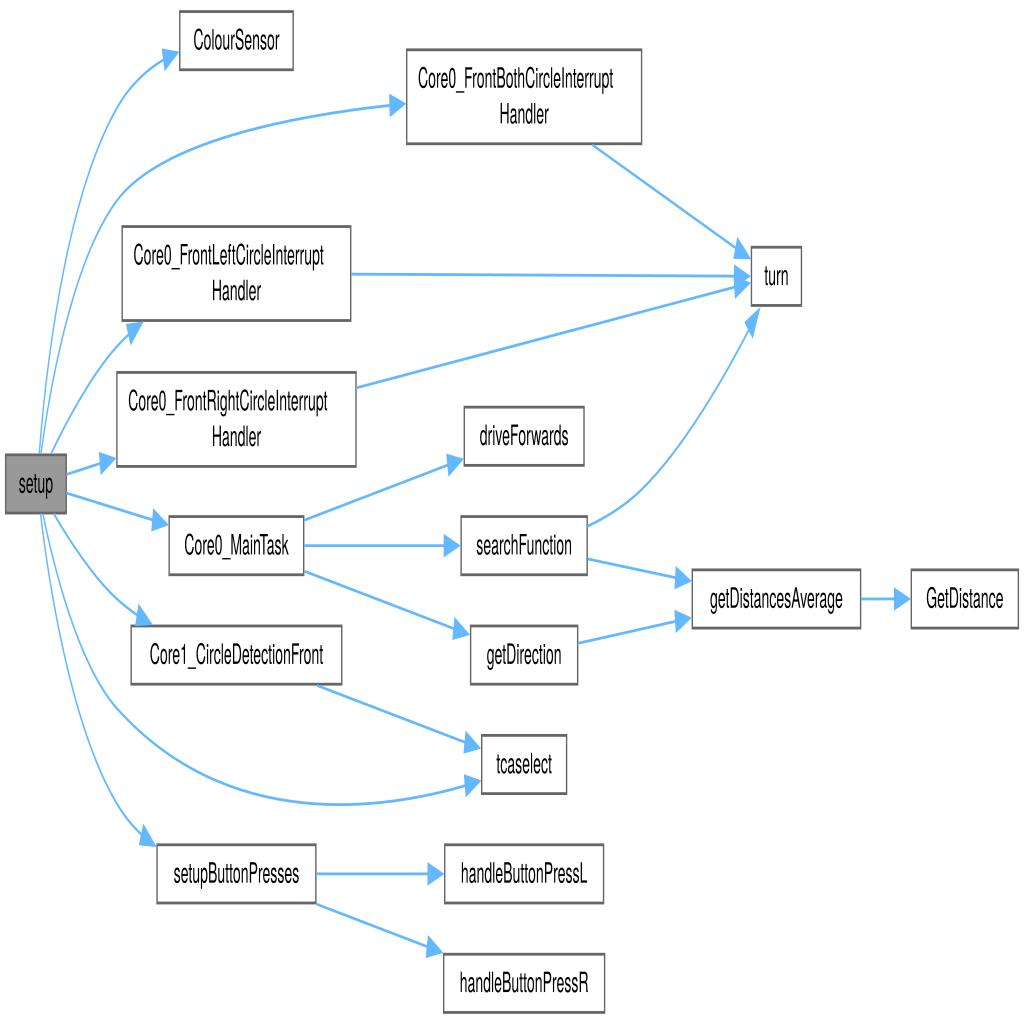
\includegraphics[width=.9\linewidth]{../callgraph.png}
\caption{Software Call Graph}
\end{figure}
\subsubsection*{Strategy}
\label{sec:org07caea3}
KillDozer uses both of the TTGO's cores, with one (core 1) checking the RGB sensors if the robot is nearing the edge of the circle, and the other (core 0) doing everything else. Core 1 will interrupt the first core's task(s), prioritising moving the robot to safety/telling the robot where to move to next.\\

The main core has a simple program loop - when it starts, it first calls the \texttt{searchFunction()}, which makes the robot turn until it detects an object closer than 1.6 meters away.
Once this happens, the function returns, and then the main function loops over a set of instructions that tells the robot to drive forwards (if one sensor is closer to the opponent than the other, then it drives forwards with a slight bias towards that direction). This continues until the RGB sensors detect the edge, at which point Core 1 interrupts this task (and sets a flag to break the while loop).\\

The interrupt handler running on Core 0 then handles the movements for the robot to take - if only one sensor is detecting the edge of the circle, the robot turns towards that sensor, until both sensors are touching (this is all done by Core 1 interrupts, using the sensor, so only one core is interfacing with the I2C bus). Turning so both are detecting the edge of the circle is done so that the opponent is definitely pushed out of the circle. Once both sensors are at the edge, the robot turns around 90 degrees, and restarts it's main looping task on Core 0, searching for another opponent.\\

We ran out of time to implement the ToF sensor, but this would have been used to detect if the opponent was inside of the bulldozer blade.\\


Using both cores meant that the robot could react immediately to a detection of going outside of the circle, whereas if we were using a single core, we could still use the task based approach to allow for interrupts, but we would not always be able to be checking the sensors, meaning that the robot could possibly go outside of the circle before it could react.
\begin{listing}[htbp]
\begin{Code}
\begin{Verbatim}
\color{EFD}\EFt{void} \EFf{Core1\_CircleDetectionFront}\EFrda{(}\EFt{void} *\EFv{pvParameters}\EFrda{)} \EFrda{\{}
  \EFk{for} \EFrdb{(};;\EFrdb{)} \EFrdb{\{}
    \EFt{float} \EFv{rFR}, \EFv{gFR}, \EFv{bFR}, \EFv{rFL}, \EFv{gFL}, \EFv{bFL};
    \EFt{float} \EFv{totalFR}, \EFv{totalFL};
    tcaselect\EFrdc{(}FRONT\_RIGHT\_TCS\_I2C\_NUMBER\EFrdc{)};
    tcs\_FR.getRGB\EFrdc{(}\&rFR, \&gFR, \&bFR\EFrdc{)};
    tcaselect\EFrdc{(}FRONT\_LEFT\_TCS\_I2C\_NUMBER\EFrdc{)};
    tcs\_FL.getRGB\EFrdc{(}\&rFL, \&gFL, \&bFL\EFrdc{)};
    totalFR = rFR + bFR + gFR;
    totalFL = rFL + bFL + gFL;

    \EFk{if} \EFrdc{(}totalFR < 350 \&\& totalFL < 350\EFrdc{)} \EFrdc{\{} \EFcd{//} \EFc{both are probably not white}
      \EFt{BaseType\_t} \EFv{xHigherPriorityTaskWoken} = pdFALSE;
      xTaskNotifyFromISR\EFrdd{(}interruptHandlerHandleBoth, 0, eNoAction,
                         \&xHigherPriorityTaskWoken\EFrdd{)};
      \EFk{if} \EFrdd{(}xHigherPriorityTaskWoken\EFrdd{)}
        portYIELD\_FROM\_ISR\EFrdd{(}\EFrdd{)};
    \EFrdc{\}} \EFk{else} \EFk{if} \EFrdc{(}totalFR < 350\EFrdc{)} \EFrdc{\{}
      \EFt{BaseType\_t} \EFv{xHigherPriorityTaskWoken} = pdFALSE;
      xTaskNotifyFromISR\EFrdd{(}interruptHandlerHandleFR, 0, eNoAction,
                         \&xHigherPriorityTaskWoken\EFrdd{)};
      \EFk{if} \EFrdd{(}xHigherPriorityTaskWoken\EFrdd{)}
        portYIELD\_FROM\_ISR\EFrdd{(}\EFrdd{)};
    \EFrdc{\}} \EFk{else} \EFk{if} \EFrdc{(}totalFL < 350\EFrdc{)} \EFrdc{\{}
      \EFt{BaseType\_t} \EFv{xHigherPriorityTaskWoken} = pdFALSE;
      xTaskNotifyFromISR\EFrdd{(}interruptHandlerHandleFL, 0, eNoAction,
                         \&xHigherPriorityTaskWoken\EFrdd{)};
      \EFk{if} \EFrdd{(}xHigherPriorityTaskWoken\EFrdd{)}
        portYIELD\_FROM\_ISR\EFrdd{(}\EFrdd{)};
    \EFrdc{\}}
    vTaskDelay\EFrdc{(}20\EFrdc{)};
  \EFrdb{\}}
\EFrda{\}}

\end{Verbatim}
\end{Code}
\caption{The task running on Core 1, which handles the edge detection sensors/logic}
\end{listing}
\clearpage
\subsection*{Bill Of Materials}
\label{sec:org6fe6ef0}
\begin{table}[htbp]
\caption{Reasoning beheind sensor choices for KillDozer}
\centering
    \begin{tabularx}{\textwidth}{|X|X|X|X|X|X|}
    \hline
        \rowcolor{CtpOverlay1}
 \textbf{Model Number} & \textbf{Part Name} & \textbf{Supplier} & \textbf{Quantity} & \textbf{Price per part (\$)} & \textbf{Cost (\$AUD)} \\ \hline
        MDD3A  & DUAL CHANNEL Motor Driver Board & Cytron & 1 & 8.5 & 8.5 \\ \hline
        ZGY370 & Worm Gear Motor & Aliexpress  & 2 & 4.49 & 8.98 \\ \hline
        TCS34725 & RGB Colour Sensor  & Aliexpress  & 2 & 2.4 & 4.8 \\ \hline
        TCA9548A & I2C Multiplexer Board  & Aliexpress  & 1 & 2.14 & 2.14 \\ \hline
        T100/T400  & Caterpillar Chain Track Pedrail Wheel  & Aliexpress  & 2 & 1.55 & 3.1 \\ \hline
        URM09  & Ultrasonic distance sensor  & DFROBOT & 2 & 7.9 & 15.8 \\ \hline
        VLX530 & Time of Flight (ToF) Laser Ranging Sensor & Aliexpress  & 1 & 1.55 & 1.55 \\ \hline
        PCB & Prototype PCB Board 9x15cm Single-Sided  & Aliexpress  & 1 & 0.31 & 0.31 \\ \hline
        OPY FLEX1K01 & Filament  & Aliexpress  & 1 & 3.9 & 3.9 \\ \hline
        M3 & Stainless Steel Cap Head bolts (10pcs) & Maker Store  & 1 & 0.252 & 0.252 \\ \hline
        IBUW & Dupont Jumper Wire Kit 40-pin 20cm & Aliexpress  & 1 & 0.517 & 0.517 \\ \hline
        \rowcolor{CtpOverlay1} FINAL PRICE & ~ & ~ & ~ & ~ & 49.8 \\ \hline
    \end{tabularx}
\end{table}
\end{document}
